\begin{center}
{\textbf{Samedi 21 août : Les cours reprennent}}
\end{center}
\vspace{2mm}

Après l’après-midi détente du 20 août, les élèves reprennent les cours pendant que les nouveaux animatheurs arrivent au compte-goutte tout au long de la journée. Les groupes A et B travaillent sur la divisibilité le matin, pendant que Théo présente les polynômes au groupe C et Martin les milieux de segments au groupe D.

On enchaîne avec au programme l’après-midi le principe des tiroirs (oui oui, c’est des maths) pour les groupes B et A, enseigné respectivement par Angela -qui donne son tout premier cours !- et Victor. Le groupe C révise les notions de puissance d’un point et le groupe D s’amuse avec des graphes.

Les élèves ont ensuite pu assister à une conférence de Jean sur les équations approchées ainsi que la présentation de la plupart des nouveaux animatheurs.

\begin{figure}[H]
\centering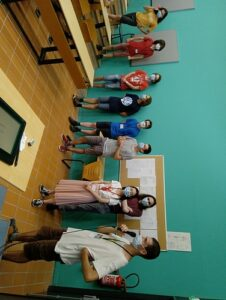
\includegraphics[width=6cm]{CR-21-0.jpg}
\caption{De gauche à droite: Yaël, Vladimir, Savinien, Colin, Antoine, Baptiste, Angela, Jean et Mathieu (devinez qui manque !)}
\end{figure}

Pour clore la journée, certains révèlent leur talent de chanteur lors de la soirée karaoké qui prend place dans l’amphithéâtre. D’autres préfèrent partir faire des jeux de société en attendant l’heure du couvre-feu.

\begin{figure}[H]
\centering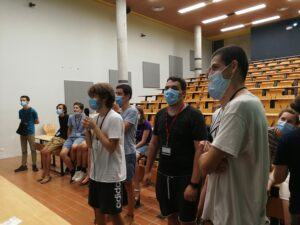
\includegraphics[width=6cm]{CR-21-1.jpg}\hspace{2cm}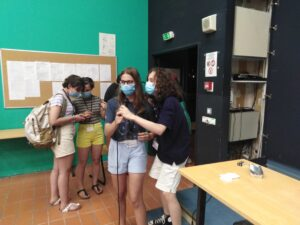
\includegraphics[width=6cm]{CR-21-2.jpg}
\caption{Les animatheurs poussent la chansonnette… et les élèves aussi !}
\end{figure}